% 서울대학교 협동과정:인지과학전공 석사ㅡ 박사 학위논문
% LaTeX 양식 샘플
\RequirePackage{fix-cm} % documentclass 이전에 넣는다.
% oneside : 단면 인쇄용
% twoside : 양면 인쇄용
% ko : 국문 논문 작성
% master : 석사
% phd : 박사
% openright : 챕터가 홀수쪽에서 시작
\documentclass[oneside,master]{snueethesis}

%%%%%%%%%%%%%%%%%%%%%%%%%%%%%%%%%%%%%%%%
%% 목차 양식을 변경하는 코드
%% subfigure (subfig) package 사용 여부에 따라
%% tocloft의 옵션을 다르게 지정해야 한다.
%\usepackage[titles,subfigure]{tocloft} % when you use subfigure package
\usepackage[titles]{tocloft} % when you don't use subfigure package
\makeatletter % don't delete me
\if@snu@ko
	\renewcommand\cftchappresnum{제~}
	\renewcommand\cftchapaftersnum{~장}
	\renewcommand\cftfigpresnum{그림~}
	\renewcommand\cfttabpresnum{표~}
\else
	\renewcommand\cftchappresnum{Chapter~}
	\renewcommand\cftfigpresnum{Figure~}
	\renewcommand\cfttabpresnum{Table~}
\fi
\makeatother % don't delete me
\newlength{\mytmplen}
\settowidth{\mytmplen}{\bfseries\cftchappresnum\cftchapaftersnum}
\addtolength{\cftchapnumwidth}{\mytmplen}
\settowidth{\mytmplen}{\bfseries\cftfigpresnum\cftfigaftersnum}
\addtolength{\cftfignumwidth}{\mytmplen}
\settowidth{\mytmplen}{\bfseries\cfttabpresnum\cfttabaftersnum}
\addtolength{\cfttabnumwidth}{\mytmplen}
%% 목차 양식을 변경하는 코드 끝
%%%%%%%%%%%%%%%%%%%%%%%%%%%%%%%%%%%%%%%%

%%%%%%%%%%%%%%%%%%%%%%%%%%%%%%%%%%%%%%%%
%% 다른 패키지 로드
%% http://faq.ktug.or.kr/faq/pdflatex%B0%FAlatex%B5%BF%BD%C3%BB%E7%BF%EB
%% 필요에 따라 직접 수정 필요
\ifpdf
	\input glyphtounicode\pdfgentounicode=1 %type 1 font사용시
	%\usepackage[pdftex,unicode]{hyperref} % delete me
	\usepackage[pdftex]{graphicx}
	%\usepackage[pdftex,svgnames]{xcolor}
\else
	%\usepackage[dvipdfmx,unicode]{hyperref} % delete me
	\usepackage[dvipdfmx]{graphicx}
	%\usepackage[dvipdfmx,svgnames]{xcolor}
\fi
%%%%%%%%%%%%%%%%%%%%%%%%%%%%%%%%%%%%%%%%

\usepackage{lipsum} % lorem ipsum
\usepackage{nameref}
\usepackage{graphicx}

%% \title : 22pt로 나오는 큰 제목
%% \title* : 16pt로 나오는 작은 제목
\title{Active Long Fixation \\
Correlates with the Formation of \\
Long-Term Memory}
\title*{적극적 장기 응시와 장기 기억 형성과의 관련성 연구}

%% 저자 이름 Author's(Your) name
%\author{홍길동}
%\author*{홍~길~동} % Insert space for Hangul name.
\author{김진화}
\author*{김~진~화} % Same as \author.

%% 학번 Student number
\studentnumber{2011-20084}

%% 지도교수님 성함 Advisor's name
%% (?) Use Korean name for Korean professor.
%\advisor{홍길동}
%\advisor*{홍~길~동} % Insert space for Hangul name.
\advisor{장~병~탁}
\advisor*{장~병~탁}

%% 학위 수여일 Graduation date
%% 표지에 적히는 날짜.
%% 학위 수여일이 아니라 논문 발간년도를 적어야 할 수도 있음.
%\graddate{2010~년~2~월}
\graddate{2015~년~2~월}

%% 논문 제출일 Submission date
%% (?) Use Korean date format.
\submissiondate{2014~년~11~월}

%% 논문 인준일 Approval date
%% (?) Use Korean date format.
\approvaldate{2014~년~12~월}

%% Note: 인준지의 교수님 성함은
%% 컴퓨터로 출력하지 않고, 교수님께서
%% 자필로 쓰시기도 합니다.
%% Committee members' names
\committeemembers%
{김~청~택}%
{장~병~탁}%
{박~주~용}%
{}%
{}%

%% Length of underline
%\setlength{\committeenameunderlinelength}{7cm}

\begin{document}
\pagenumbering{Roman}
\makefrontcover
\makefrontcover
\makeapproval

\cleardoublepage
\pagenumbering{roman}

\begin{abstract}
The application of eyewear accelerates the study on the eye movement, for the eye movement is a non-invasive and convenient indicator of the brain activities. We investigate the eye movements of the subjects watching the kids video. We analyze the video sequences by classifying them into two different sequence groups that have the long and short fixation duration, respectively. First, we conduct the long-term memory test of whether fixation duration correlates with long-term memory. Second, we classify its visual constraints into alert and no alert types. As a result of the test, the fixation duration itself is not decisive. However, the long fixations which are actively engaged with alert type movie clips statistically have higher scores, while the short fixations do not. Finally, we propose a simple computational model using the linear regression of two significant features, saliency scrutiny and fixation duration. It may provide an explanatory way to the efficient memory mechanism for the life-long sequences.

\keyword{Eye movement, fixation, spatio-temporal, long-term memory, computational modeling}

\end{abstract}

\tableofcontents
\listoffigures
\listoftables

\cleardoublepage
\pagenumbering{arabic}

\chapter{Introduction}

The brain is the most intelligent organ in a living thing. It receives many different forms of sensory information and processes this information appropriately with regard to its survival and reproduce. Especially, the visual information takes a very special position among other kinds of sensory information as it does not need to sense a source directly but is transfered to a remote target far freely than any other types of the sense. Furthermore it gives more chances to survive in the situation of being threaten by the predators using their eyes to detect the foes in the remote place before their approaching. 

But this notable advantage is not freely given to one as it requires more delicate and clever way of interpreting the visual information. Because the visual information can easily be affected by the moment-to-moment environmental changes, heuristic but robust compensation strategies are required. Hence, how the brain processes the visual information provides the profound way to study the mechanism by which the brain precisely and efficiently processes the most dynamic and enormous sensory information.

There are a lot of studies on the computational modeling for the visual information, which include the visual fragment completion, the scene or object classification and recognition \cite{winn2005,lazebnik2006}, and object tracking \cite{YiWu2013}. These research topics often tend to focus on the objective for each task, not on the implementation of the method how the brain deals with the visual information. As a result, the computational approach to the modeling for the visual information processing of the brain is gradually changed to the optimization problem, which hinders the understandings of the human-level information processing abilities. 

Particularly, the object tracking seems to describe how we pay attention to an interesting object, however, the eye movement, mostly controlled by the oculomotor system, complicates with how the brain works for the acquisition of the visual information \cite{Henderson2003}. For instance, in the fixation state, the human eyes only recognize the small portion of the whole sight. If you read this paper from an 8-inch distance fixing on one particular letter, you cannot read outside of next two words or about ten letters which are presented in the para-fovea. Since the brain is well-known for its parallel processing on the neural circuits, this sequential notion of eye movement for the visual system would be inefficient for information processing. Therefore, we should notice that the experimental results of covert attention and shifting receptive field are also the important subject to study \cite{Zirnsak2014}.

The studies on the reading eye movement, which are relatively well studied by psychologists and neuroscientists \cite{Rayner1998,Reichle1998}, reveal that fixation duration is related to the presence of the cognitive process \cite{Rayner1997}, such as observing its correlation with linguistic attributes \cite{Inhoff1986,Rayner1986}.

There is a different aspect in studying the eye movement for video stimuli. The duration of fixation is more constrained by the affective content, such as emotional response, including a context of it, compared to the reading materials. Moreover, the selection of the next fixation and the direction of a saccadic movement tend to be more liberal than the dominance of horizontal searching in reading. 

Therefore, the study of the eye movement on the video stimuli has been neglected due to the complexity of the research and the methodological difficulties \cite{Tatler2011}. However, the recent advancement of the sensory device, like the Google Glass and the mobile devices for eye tracking, promotes studies on the video stimuli and in natural experimental environment, to apply the research models or applications on mobile devices. 

We investigate the characteristics of eye movements on the video stimuli focusing on the formation of long-term memory using recognition test. The basic elements of the eye movements are segregated into the fixation duration and the saccade vector, which consists of the saccade direction and the length of the saccadic movement \cite{Findlay1999,Feng2006}. In this study, we focus on the characteristics of the fixation duration as the evidence of the cognitive process to memorize. Moreover, as the movie clips which potentially induce emotional arousal are known to increase the recognition of the previously watched movie clips \cite{Cahill1996amyg,Cahill1998baso}, we will see if the arousal effect is asserted by the duration of fixation. Finally, we propose a linear regression model based on the active features of eye movement, saliency scrutiny and fixation duration.



\chapter{Materials and Methods}
\label{sec:material-and-methods}


\section{Study 1}

For this study, we prepared the video material \textit{Pororo Season 3}, which is a famous kids video in Republic of Korea. In this video, there are artificial 3D-rendered characters and other objects who have distinctive traits, so visual features are easily captured by eye movements. \textit{Pororo Season 3 DVD 1} contains 13 consecutive episodes, each with a different single storyline. The total playing time is 67 minutes and 50 seconds.

We recruited 18 participants with normal vision (11 males, 7 females; 23-31 age), who are graduate students in Seoul National University, voluntarily participated in the study. For the stability of collecting data and the eye gear requires appropriate head circumference, we chose the target participants for this study. All participants had not experienced a brain damage or a behavioral disorder. The participants were first time viewers of the video, \textit{Pororo Season 3}. To prevent distraction, each participant took a set of tests for the two-split video, one is about 32 minutes of the first half and the other is about 36 minutes of the later half, each on the other day. Later then, we merged two parts into one manually, in a way that the results do not overlap. 

Participants watched the kids video in the room which has the experimental settings. The room is about 3 square meters surrounded by the opaque curtains. On the side of the room, a wide-screen HDTV (1920x1080 resolution, 885 mm x 500 mm, 16:9 ratio) was installed, and 2.1 channel speakers. Participants were guided to sit on a comfortable sofa in front of 1.7 m from the TV screen.

Concurrently, the eye movements and the user-perspective scenes were recorded by \textit{Tobii Glasses eye tracker}, the corneal reflection based system with a sampling rate of 30 Hz. We used the \textit{I-VT algorithm} as the fixation filter (system default), which classified fixations with the velocity threshold of 30 degree per second. Usually, the saccadic eye movements are discriminated with low velocities (less than 100 degree/second) and high velocities (higher than 300 degree/second), in which the velocity-based classification is a simple and reasonable approach \cite{Salvucci2000}.

We classified the event types of the eye movements into three categories; fixation, saccade and unclassified. The unclassified data were discarded and not used in this study.


\section{Study 2}

For 11 participants who have participated in \textit{Study 1}, we prepared the controlled memory test for each participant. We conducted this study 3-4 months after the \textit{Study 1} (the intervals are not consistent due to schedule conflicts). A memory test consisted of total 20 movie clips; 8 movie clips for long fixations, another 8 movie clips for short fixations, and the remaining 4 movie clips for the control, which were not seen in the previous study. In detail, the lengths of all movie clips were each 3-second long. \textit{The long fixation sequences} were randomly picked from each participant's data containing the fixation longer than 1400 ms in the middle of the movie clip. \textit{The short fixation sequences} were randomly picked from each participant's data containing the fixation shorter than 300 ms. The 4 control movie clips were randomly picked from the other season of \textit{Pororo} series, \textit{Pororo Season 2}.

Each participant identified 20 movie clips that were sorted randomly. Each participant gave a score for each movie clip between 1 and 5, which is an integer, depending on the assurance of whether he or she saw the movie clip before or not. Notice that, in this study, 1 is the lowest score, not 0, which means that the movie clip is surely not seen.


\chapter{Fixation Duration}
\label{sec:fixation-duration}

Fixation duration takes an important position in reading task, because the durations of eye fixations seems to be constrained by the linguistic features of the fixated word \cite{Rayner1986,Inhoff1986}. In the video watching task, we anticipated the characteristics of fixation duration to be different from those in the reading task. As expected, the fixation duration was changed more drastically, up to 10 seconds during watching the video. These changes were partly caused by the sequential changes of the visual stimuli and the fluctuated responses of the oculomotor system and cognitive processes. We assumed the fixation duration as a random variable with probabilistic distribution \cite{Rayner1998,Reichle2004,Reichle2006}, because the length of fixation duration is not a deterministic property, and more than a single component dynamically contribute to the final motor command and the execution for the oculomotor system.


\section{Marginal Distribution of Fixation Durations}

Figure~\ref{fig:marginal-fixation-duration} shows the marginal distribution of fixation durations, which includes all of the 158,643 fixation durations of 18 participants. The x-axis represents the duration time, and the y-axis represents the log scale of the number of fixations across the whole data.

\begin{figure}
  \centerline{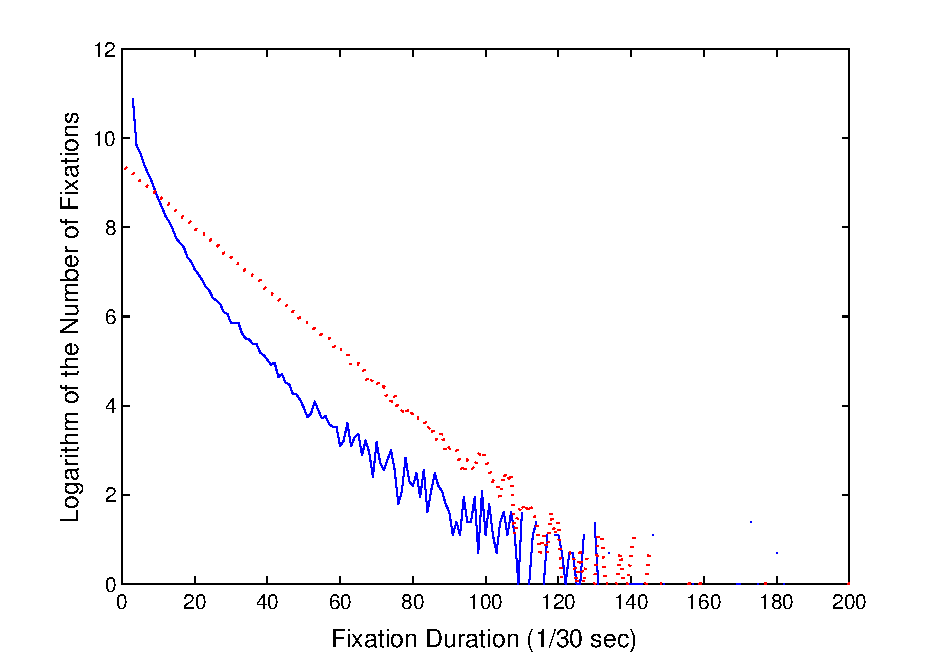
\includegraphics[width=150mm,height=110mm,trim=0mm 60mm 0mm 60mm]{./eps/marginal_fixation_duration.pdf}}
  \caption[The marginal distribution of fixation durations]{The marginal distribution of fixation durations. All of the 158,643 fixation durations of 18 participants was used. The x-axis represents the number of time unit, 1/30 sec., therefore, 30 indicates 1 second. The y-axis represents the logarithm of the number of fixations which have the same time length with regard to the time unit of x-axis.}
  \label{fig:marginal-fixation-duration}
\end{figure}

The shape of the marginal distribution of fixation durations (Figure~\ref{fig:marginal-fixation-duration}) is roughly illustrated as an exponential function. The distribution of the \textit{reading} fixation durations has a quiet different shape \cite{Feng2006}, segmented into three parts, slow-rising ones for short fixations, fast-rising period until around 180 ms, and following a long tail for long fixation durations. These facts allow us to think that 180 ms of the fixation duration for reading is the most general case, but obviously not for watching the video.

Fixation durations which were longer than about 2 seconds are getting more unpredictable along with increasing the fixation duration. Though it is due to the logarithm increasing the sampling variance, occasionally the content of the video stimuli determined how long the eye gaze was fixated. In other words, the fixation more tends to maintain the gaze position when the visual constraint is imposed. The visual constraints had various forms, and it will be discussed in Section~\nameref{subsec:Long-Fixation-Durations}.


\section{Individual Distributions of Fixation Durations}

Interpersonal differences were also examined. The individual distributions of fixation durations are shown in Figure~\ref{fig:individual-fixation-duration}. The medians of fixation durations from all 18 participants varies from 133 ms to 267 ms with the mean of 183.3 and the standard deviation of 41.7. For the analysis, we randomly selected 8 participants' data in Figure~\ref{fig:individual-fixation-duration}. 


\begin{figure}
  \centerline{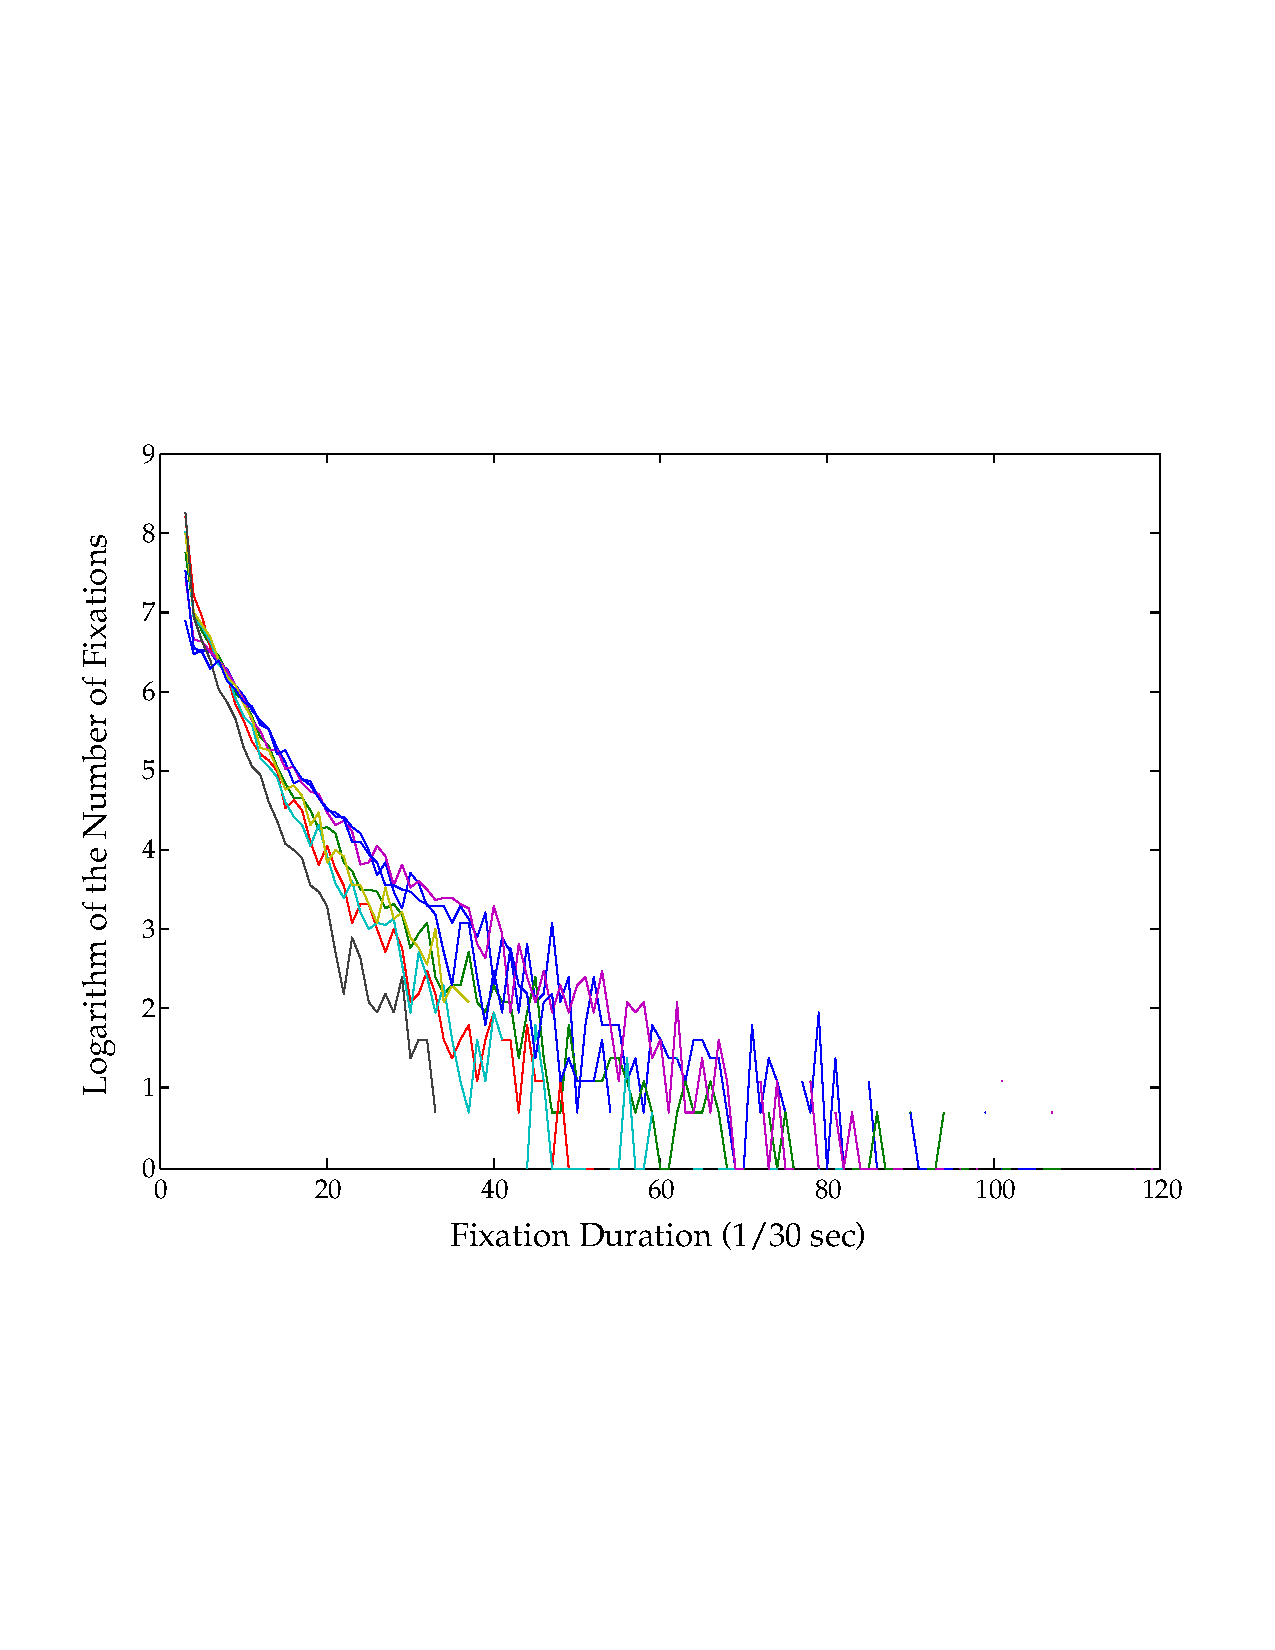
\includegraphics[width=150mm,height=110mm,trim=0mm 60mm 0mm 60mm]{./eps/individual_fixation_duration.pdf}}
  \caption[The distribution of fixation durations for individuals]{The distribution of fixation durations for the randomly selected 8 participants. We found the interpersonal differences among all 18 participants, the median of fixation durations varies from 133 ms to 267 ms (mean=183.3, std=41.7).}
  \label{fig:individual-fixation-duration}
\end{figure}


\section{Long Fixation Durations}
\label{subsec:Long-Fixation-Durations}

In Figure~\ref{fig:long-fixations} the sequences of frames which received more than 2 seconds of the fixation duration from at least 3 different participants are shown. We set the threshold to reduce the interpersonal variation. We got all 41 sequences across 1 hour 7 minutes 50 seconds length of the material. For the review, we chose 10 typical sequences. Each row represents an independent sequence and each column shows a single frame. The time interval between the frames is 0.5 seconds. The colored dots represent the fixation positions, whose durations are longer than 2 seconds. The same color means the same participant. Four different types of the sequences are listed as \textit{alerted} (3), \textit{successive} (3), \textit{stationary} (3), and \textit{Unclassified} (1) for the review. The classification is conducted by one of authors and two other colleagues. Every sequence used by this study is classified by agreement. If there is a conflict or not fit to the major types, then the sequence is classified as \textit{Unclassified}.

\begin{figure*}
  \centerline{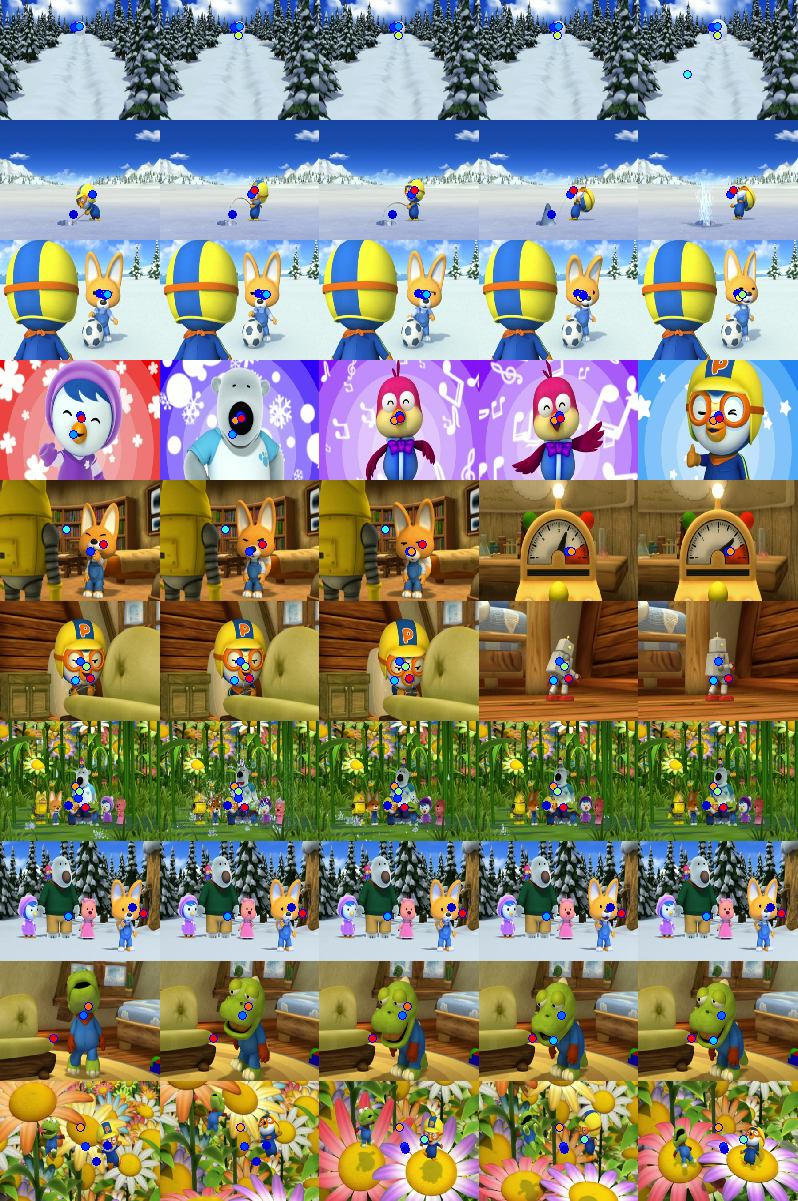
\includegraphics[width=76mm]{./eps/long_fixations_types.png}}
  \caption[The samples of sequence types]{The sequences of frames which received more than 2 seconds of fixation duration from at least 3 participants. Each row shows an independent sequence and each column shows a single frame. The time interval between frames is 500 ms. The colored dots mean the fixation positions, whose durations are longer than 2 seconds. The same color of dots means what is from the same participant. First 3 sequences show the \textit{alerted} type, then next 3 sequences show the \textit{successive} type, then next 3 sequences show the \textit{stationary} type, and then the last sequence shows the \textit{Unclassified} type of visual constraints for the review. For the description of those sequences, see the text in Section~\textit{\nameref{subsec:Long-Fixation-Durations}}.}
  \label{fig:long-fixations}
\end{figure*}

The sequence of the \textit{alerted} type was classified because the scene implied an unusual and, potentially dangerous or difficult situation, which may introduce a mental arousal. The sequence of the first row demonstrates an urgent moment that a huge snowball is about to roll down the hill, which was previously rolled up by the robot, \textit{Rody}. Second shows that \textit{Pororo} has been fishing at the ice hole, but what he caught was \textit{Shark}, a naughty character. Third shows that \textit{Eddy} rolled his eyes to kick his ball avoiding the opponent \textit{Pororo}.

The \textit{successive} type shows that the fixation duration extends across more than 2 different scenes. Because the location of the target object is not changed or changed within the range of a foveal or central vision, 2-5$^{\circ}$, the fixation holds its position \cite{mcmorris2014acquisition}. The fourth sequence shows the closed-up characters are serially shown up in the center of the screen. The fixations duration of the fifth and sixth sequences extends across different scenes have different visual configurations.

The \textit{stationary} type most clearly shows the characteristics that the indifferent scene maintains while the target object moves a little bit or even does not move. For there is not a particular event or a change of the scene, the participants tend to fixate their gazes. See the seventh through ninth sequences.

The sequence of the \textit{Unclassified} type takes various forms. The tenth sequence shows that \textit{Pororo} and \textit{Crong} just jumped out of the shoulder of the magician dragon \textit{Tongtong}, who is flying in the sky. Two sunflowers spring \textit{Pororo} and \textit{Crong} into the sky in multiple times. But due to the perspective of the camera, the location of the two characters in the scene is almost fixed. Participants fixated their eye gazes on the center of the two characters while the background shifting up and down. In other cases, though not reported in Figure~\ref{fig:long-fixations}, there were cinematic techniques, i.e., tracking, tilt, zoom-in and zoom-out, and other uncertain ones. The number of these cases is relatively smaller than the other types, hence we classify all of them into the \textit{Unclassified}. We summarize those three typical types in Table~\ref{tab:long-fixation-types}.


\begin{table*}[htbp]
\begin{center} 
\caption{Long Fixation Types.} 
\label{tab:long-fixation-types} 
\vskip 0.12in
\begin{tabular}{lp{8cm}} 
\hline
Long fixation type    &  Description \\
\hline
Alerted         &   An urgent situation happens with an object, \\
                &   \hspace{5mm} which can be easily targeted as a cause.\\
Successive      &   Successive changes to keep attracting. \\
Stationary      &   The scene is the same while the target object(s) \\
                &   \hspace{5mm} moves a little or even does not move. \\
Unclassified    &   Cinematic techniques, which are tracking, tilt, \\
                &   \hspace{5mm} zoom-in and out, and others. \\
\hline
\end{tabular} 
\end{center} 
\end{table*}



\chapter{Long-Term Memory Formation}

In the studies of reading eye movements, as noted before, the fixation duration is a good indicator for information processing. The stimulus-response model seems to offer a way of understanding, because a sequence as a stimulus supplies a cause to response, in this case, a long fixation. Even so, we have to be cautious that the long fixation itself was not always induced when the internal state of a subject is affected. In addition, the sequences that received a long fixation did not decisively guarantee the quality of information processing nor its specificity. When we carefully look into the sequences in Figure~\ref{fig:long-fixations}, the fixations on \textit{successive} or \textit{stationary} type sequences can be interpreted as looking passively or even blankly.

This view is also valid for the formation of memory. A stimulus is memorized by the constructive activities, which is a series of stimulations, giving attention, and acquisition. Yet the corresponding responses are not deterministic by the stimulus for the uncertainty of environmental perturbations or the complexity of internal states. Therefore, the formation of memory is the result of the cognitive process of response rather than the response itself. However, the cognitive process is an internal procedure, which only can be measured by the tangible responses indirectly. So, we need to discern the reliable indicator of the cognitive process with a sufficient care.


\section{Recognition Test}

We defined two types of fixation as long and short fixations. The long fixation was defined by the gaze holding its position after fixation filtering, which is longer than 1400 ms. The short fixation was defined by the one that is shorter than 300 ms. Figure~\ref{fig:memtest-leng} shows the memory test result for the two fixation types. Each participant assessed in a recognition test rating 20 movie clips, containing 8 long fixated movie clips, 8 short fixated movie clips and 4 not-seen movie clips, which were not seen previously. Contrary to our expectations, the scores for the short fixated movie clips were not much different from the scores for the long fixated movie clips. This result makes sense considering that the long fixation is an attentive response, which can be actively or passively motivated by a reciprocal process in visual system.

The relationship between the emotional arousal and the formation of long-term memory was known for the studies in neuroscience \cite{Cahill1996amyg,Cahill1998baso}. In this study, we define that the emotionally arousal events are urgent, threat, tension, hurt, trouble, surprise or angry situations. On top of this, more detailed analyses are conducted with regard to this.

Figure~\ref{fig:memtest-long} shows the memory test result for the long fixation which was on the \textit{alert} movie clip or the \textit{no alert} movie clip. The \textit{alert} movie clips included the emotional arousal events, which was previously defined. This classification is rather definite because the content is an animation video for children. Figure~\ref{fig:memtest-alert} shows the result of arousal effect on the recognition test. \textit{Alert} movie clips significantly got higher scores than \textit{no alert} movie clips with the p-value of 0.0077 (p $<$ 0.01). The numbers of ratings from 11 participants were 19 for the \textit{alert} and 69 for \textit{no alert}. The difference between the two mean scores for the long and short fixation types was significant. The p-value of two-sample t-test was 0.0104 ($<$ 0.05). The blue horizontal line indicates the mean scores for the long fixated movie clips.

Figure~\ref{fig:memtest-short} shows the memory test result for the short fixation which was on the \textit{alert} movie clips or the \textit{no alert} movie clips. The numbers of cases from 11 participants were 21 and 67, respectively. The p-value of two-sample t-test was 0.2484 ($>$ 0.05). In the short fixation cases, there was no significance between the two content types, \textit{alert} type and \textit{no alert} type. The blue horizontal line indicates the mean scores for the short fixated movie clips.


\begin{figure*}
  \centerline{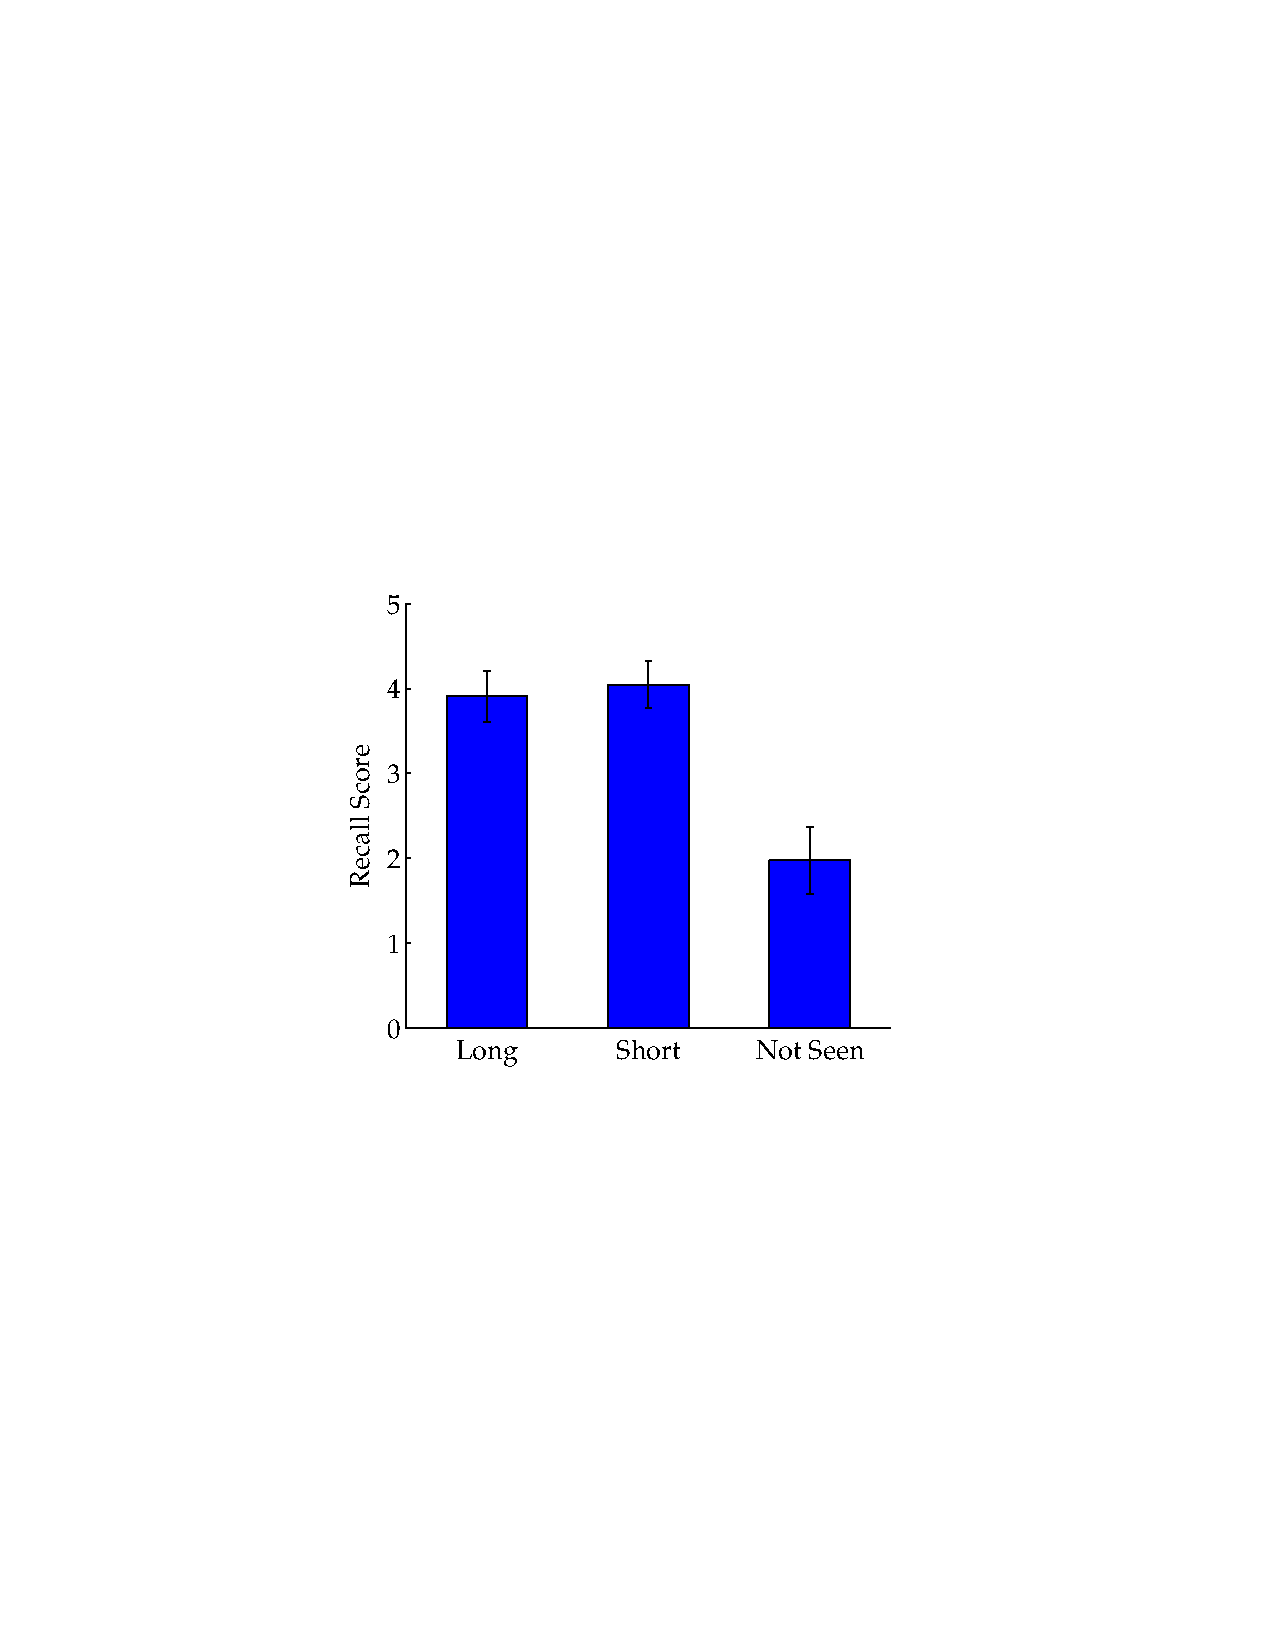
\includegraphics[width=100mm,height=94mm,trim=54mm 90mm 54mm 90mm]{./eps/memtest_leng}}
  \caption[Long-term memory test result for two fixation duration types]{Long-term memory test result for two fixation types, one is that whose duration of fixation is longer than 1400 ms, and the other one is that whose duration of fixation is shorter than 300 ms. Each participant rates 8 long fixated movie clips, 8 short fixated movie clips and 4 control movie clips which are not seen previously. Surprisingly, the mean scores of the short fixated movie clips are indifferent to the mean scores of the long fixated movie clips (p $=$ 0.5051). Error bars indicate $\pm$ 2 standard errors of means (SEMs). For the detail of test, refer to \textit{\nameref{sec:material-and-methods}}.}
  \label{fig:memtest-leng}
\end{figure*}

\begin{figure*}
  \centerline{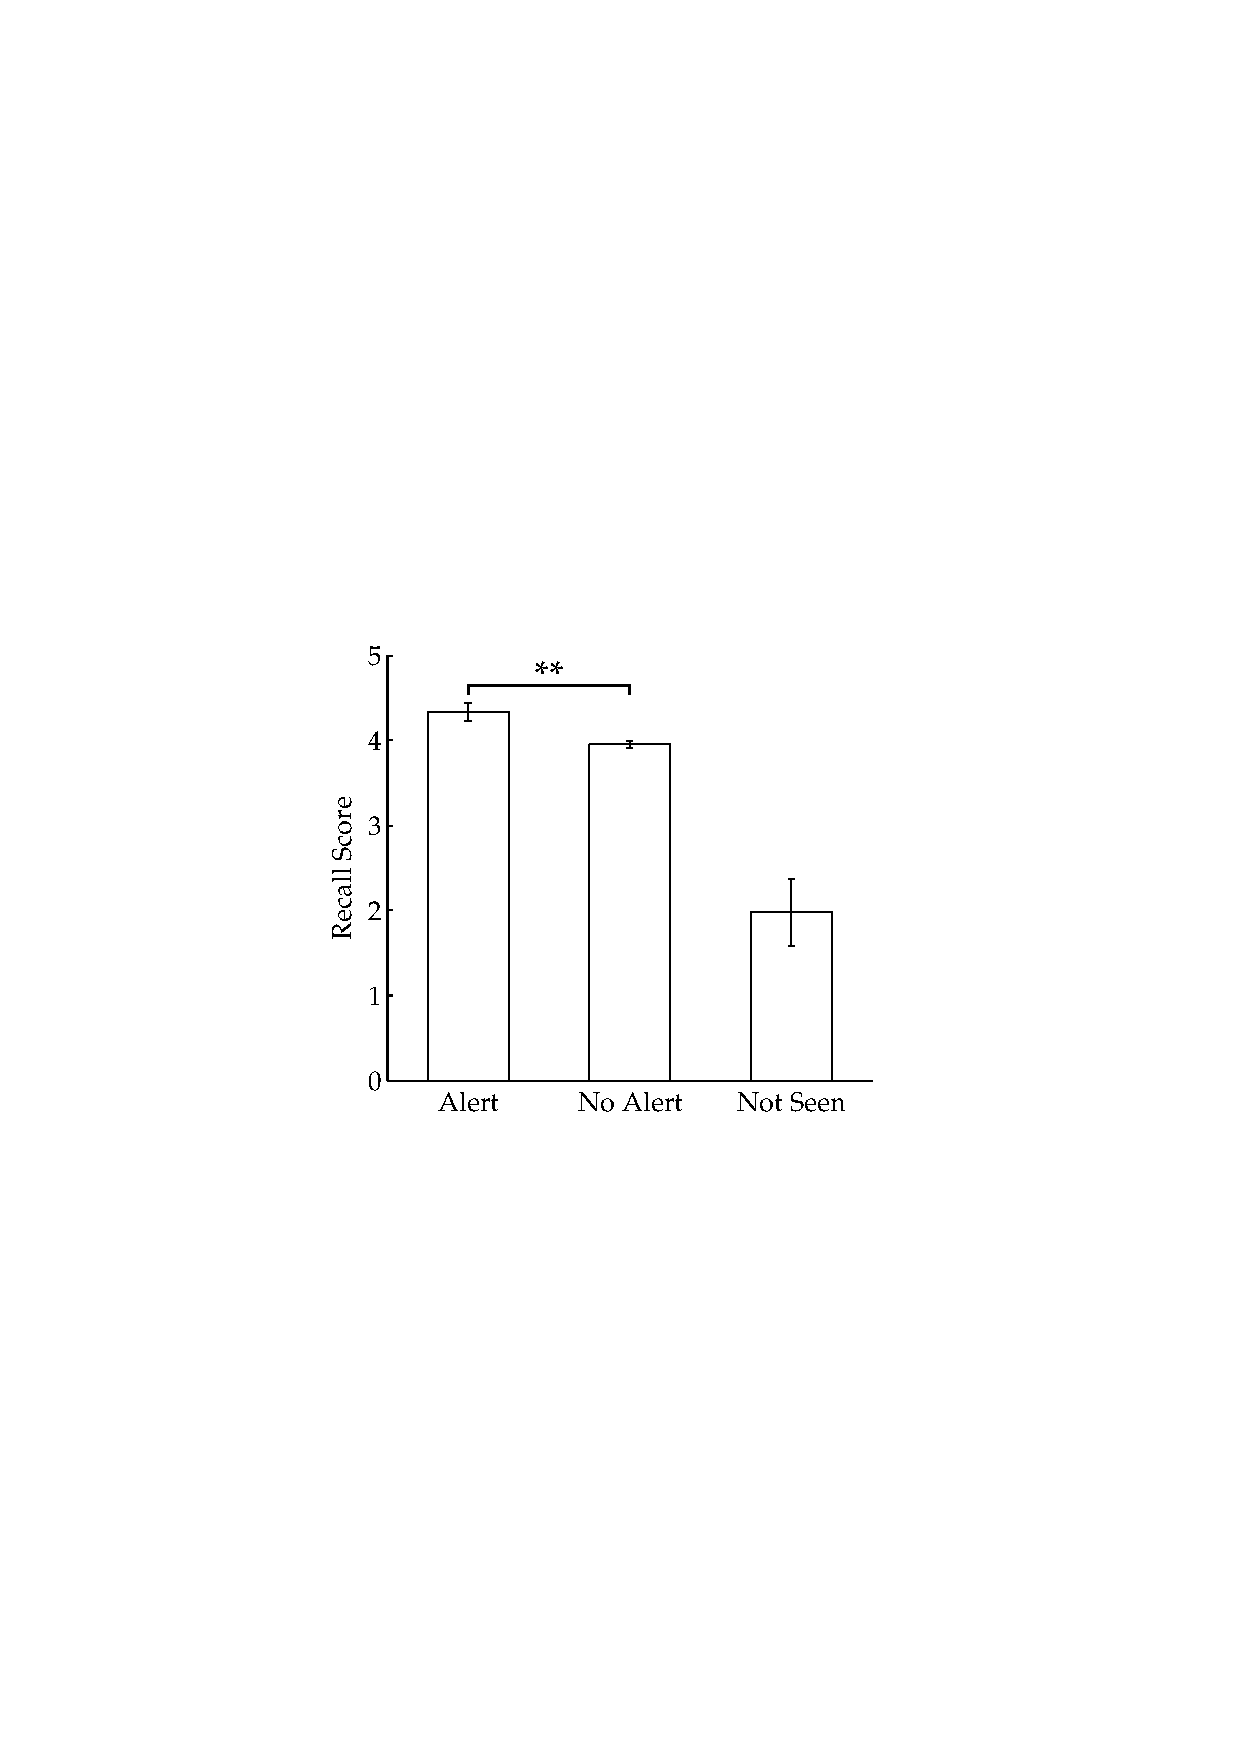
\includegraphics[width=100mm,height=94mm,trim=54mm 90mm 54mm 90mm]{./eps/memtest_alert}}
  \caption[Long-term memory test result for alert and no alert types]{Long-term memory test result for \textit{alert} and \textit{no alert} types. The arousal affects on the recognition test, alert movie clips significantly get higher scores than no alert movie clips with the p-value of 0.0077 (p $<$ 0.01). Error bars indicate $\pm$ 2 standard errors of means (SEMs).}
  \label{fig:memtest-alert}
\end{figure*}

\begin{figure}
  \centerline{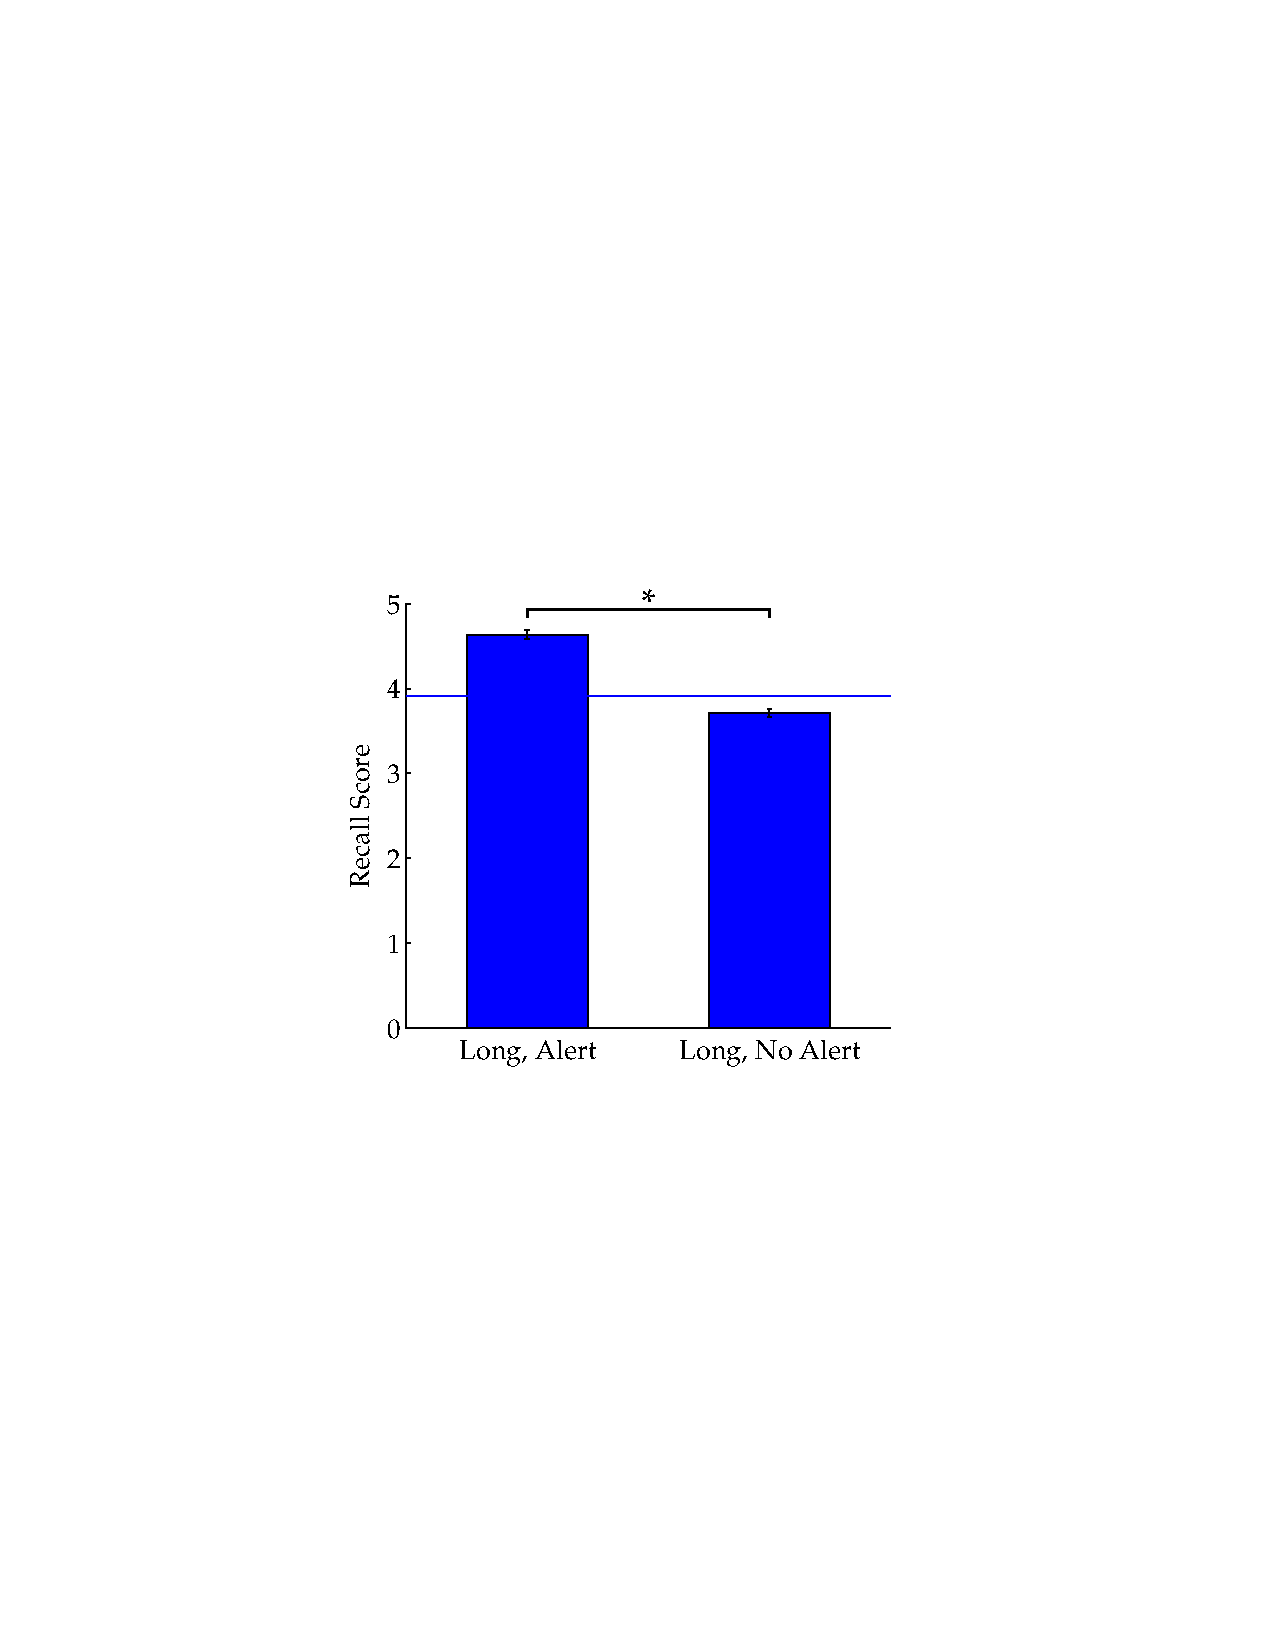
\includegraphics[width=100mm,height=94mm,trim=54mm 90mm 54mm 90mm]{./eps/memtest_long.pdf}}
  \caption[The memory test result for the long fixations which are on alert movie clips or no alert movie clips]{The memory test result for the long fixations which is on the \textit{alert} movie clips or the \textit{no alert} movie clips. The numbers of cases from 11 participants are 19 and 69, respectively. The difference between two means is statistically significant, the p-value of two-sample t-test for the \textit{alert} type is 0.0104 ($<$ 0.05). The blue horizontal line indicates the mean scores of the long fixated movie clips. Error bars indicate $\pm$ 2 SEMs.}
  \label{fig:memtest-long}
\end{figure}

\begin{figure}
  \centerline{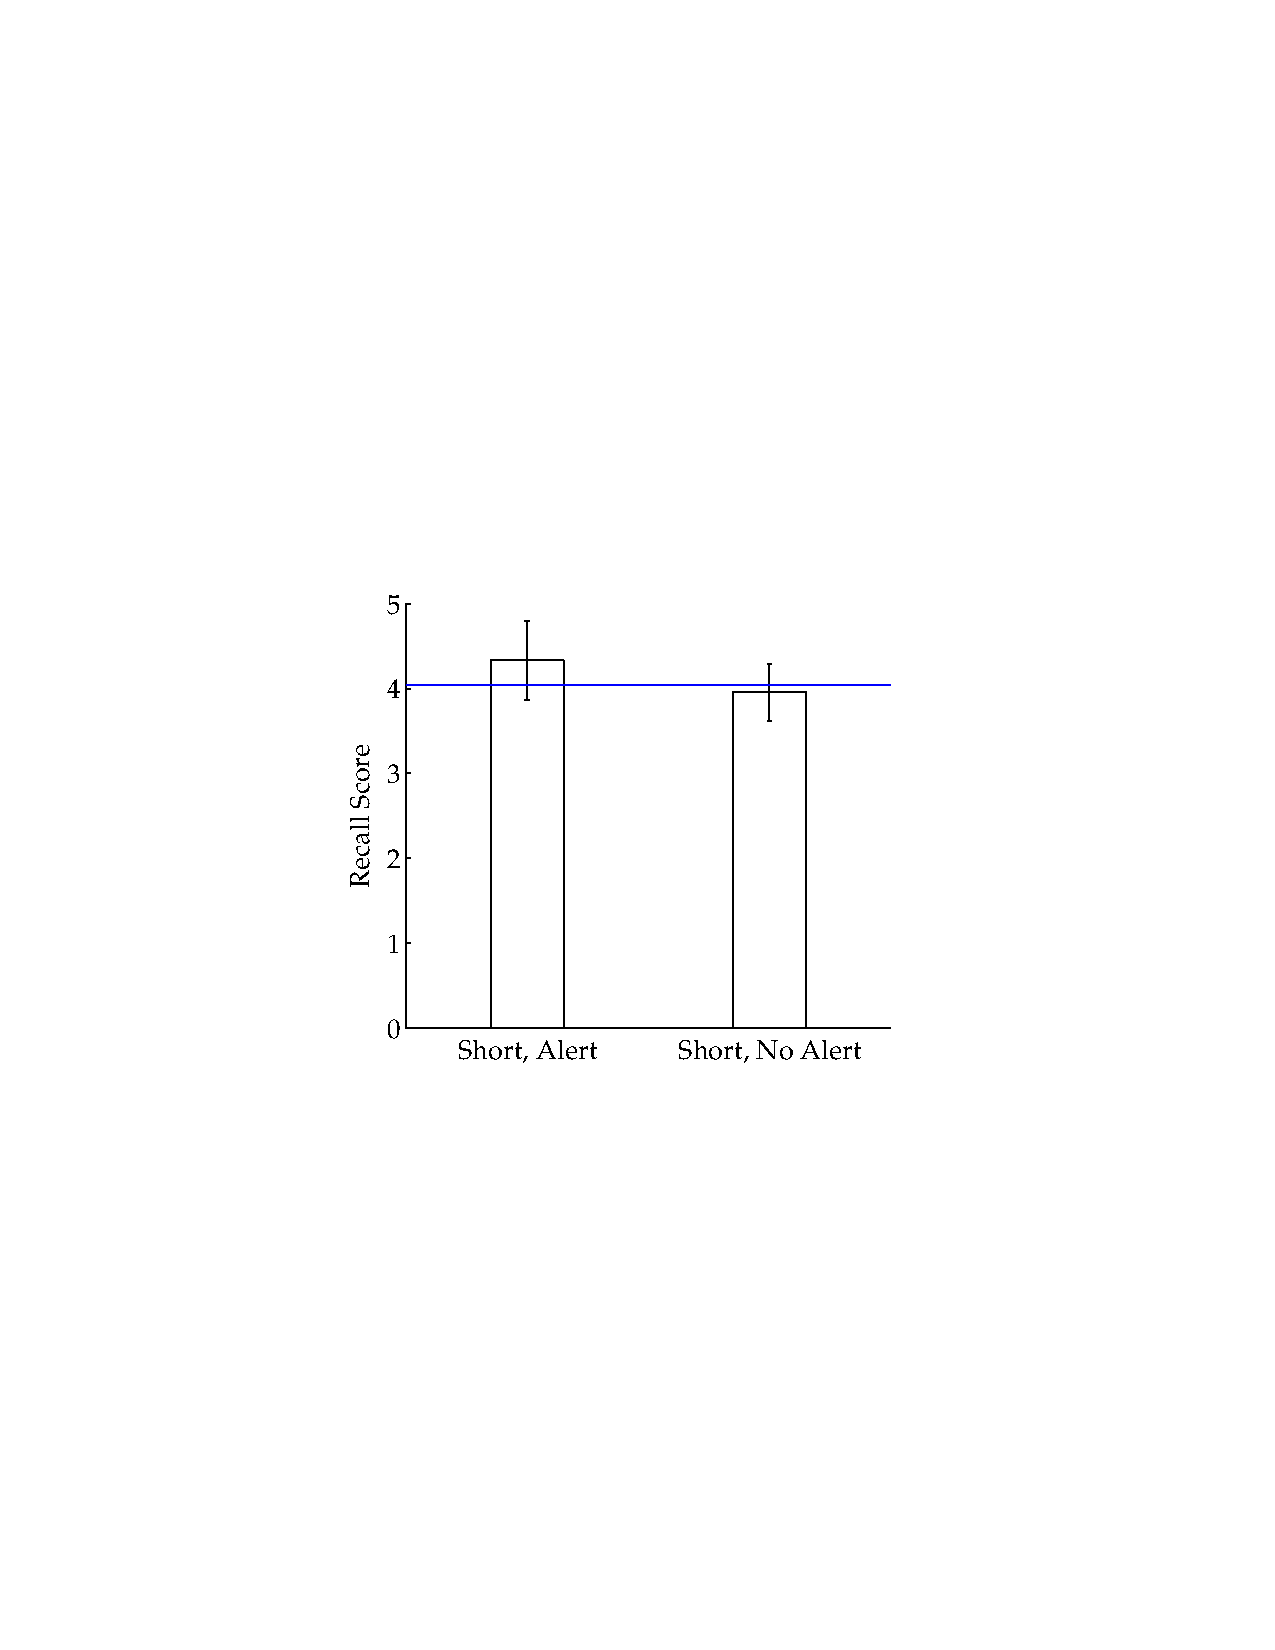
\includegraphics[width=100mm,height=94mm,trim=54mm 90mm 54mm 90mm]{./eps/memtest_short.pdf}}
  \caption[The memory test result for the short fixations which are on the alert movie clips or no alert movie clips]{The memory test result for the short fixations which is on the \textit{alert} movie clips or the \textit{no alert} movie clips. The numbers of cases from 11 participants are 21 and 67, respectively. The p-value of two-sample t-test for the \textit{alert} type is 0.2484. The blue horizontal line indicates the mean scores of the short fixated movie clips. Error bars indicate $\pm$ 2 SEMs.}
  \label{fig:memtest-short}
\end{figure}


\section{Gaze Variations}
\label{subsec:gaze-variations}

The difference of the eye movements between the \textit{alert} movie clips and the \textit{no alert} movie clips for the long fixated was observed by the variation of gazes. Actually, the gazes keep moving in the fixation state, because eye balls are fixed by twitching extraocular muscles. However, the most contribution to that variation was a smooth pursuit. In the smooth pursuit, the eyes were following a slowly moving object or interesting features. Because our experimental settings did not and can not precisely define the smooth pursuit, all the eye movements slower than 30 degree per second were candidates. 

To get the variation of the gazes excluding the variation from the smooth pursuit, we used the window sliding technique. Varying the size of a time window, we moved the time window on the time series by 1/30 second in every step, and took the median of the variations. Figure~\ref{fig:gaze-variation} shows the significant level changes according to the change of the window size. If the window size was smaller than 200 ms, p-values were lower than 0.05. In the long fixated group, the \textit{alert} movie clips tended to have smaller gaze variations than the \textit{no alert} movie clips have, whereas the short fixated group did not show these differences.

\begin{figure}
  \centerline{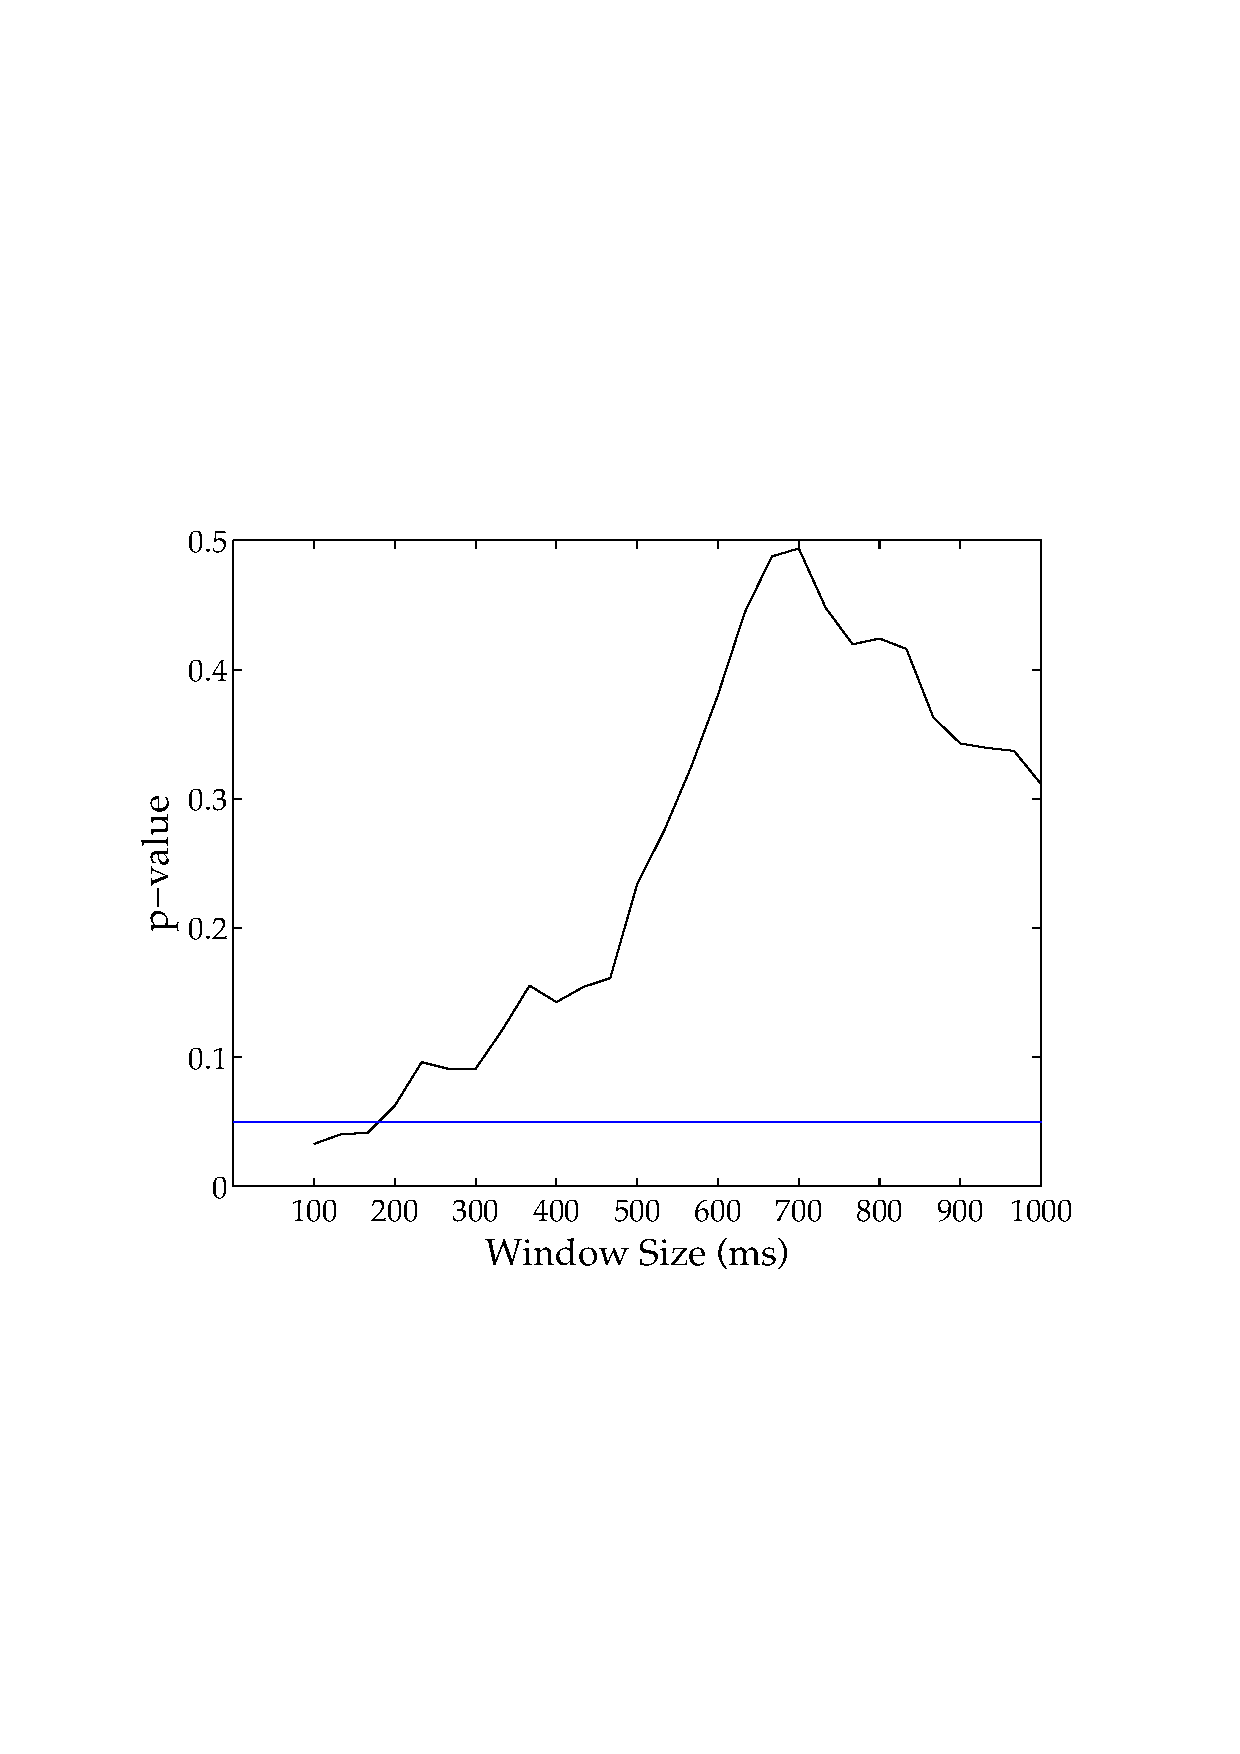
\includegraphics[width=100mm,height=95mm,trim=28mm 75mm 28mm 76mm]{./eps/gaze_var.pdf}}
  \caption[The significant levels of gaze variations with regard to the window sizes]{The significant levels of gaze variations with regard to the window sizes. When the window size is narrower than 200 ms, the medians of gaze variations for the \textit{alert} movie clips are significantly different from those for the \textit{no alert} movie clips (p $<$ 0.05). The blue horizontal line shows the 5\% significant level.}
  \label{fig:gaze-variation}
\end{figure}


\section{Computational Model}

Based on the study of bottom-up attention \cite{koch1985shifts}, the computational model was implemented by the saliency map-based approach \cite{itti1998model}. This model used the visual information, i.e., intensities, color opponencies and orientations, as a source to measure the conspicuity \cite{Parkhurst2002}. While reflecting physiological evidences for the basis mechanisms of visual information processing, active selection to increase the information gain, which is depicted as ``best question to ask'' \cite{Reinagel1999,zetzsche1998investigation}, the implement had both processing efficiency and robustness to noises. It took an image as input, and it returns one saliency map, a matrix, whose elements were normalized iteratively and nonlinearly \cite{itti2000saliency}.

Using the saliency map from the computational bottom-up attention model, we examined the association between the gaze fitness to the model and the score. The fitness function is described below. We used the SaliencyToolbox with default parameters for getting the saliency map to analyze, and aligned the gaze coordination to the area of the saliency map, which had a smaller size after sub-sampling \cite{Walther2006}.

\begin{equation}\label{eq:salsum}
X_{saliency}^{(i,j)} = \sum_{t=1}^{T} \mathcal{S}_{x_{t},y_{t}}^{(i,j,t)}
\end{equation}

In Equation~\ref{eq:salsum}, $x_{t}$ and $y_{t}$ represent the mapped gaze coordination at $t$ time in a fixation duration. $\mathcal{S}^{(i,j,t)}$ is a saliency map which is the output of the model for a given screenshot at $t$ time in the duration of a movie clip, that was given to the participant $i$ for the $j$-th movie clip of the recognition test.

We fit the parameters for the linear regression model for the scores, which was defined by Equation~\ref{eq:lm},

\begin{equation}\label{eq:lm}
Y_{score} = \mathcal{B}_{0} + \sum_{l \in \mathcal{L}} \mathcal{B}_{l} \cdot X_{l}
\end{equation}

\noindent, $\mathcal{B}$s are the coefficients of the model, and $\mathcal{L}$ is a set of features as  

\begin{equation}\label{eq:l}
\mathcal{L} = \{duration, saliency\}.
\end{equation}

$X_{duration}$ is the fixation duration in second, and $X_{saliency}$ is defined by Equation~\ref{eq:salsum}. We used only the data of the long fixations, because the short fixated movie clips did not show the significant differences on the scores for the duration and the gaze fitness to the saliency map.

\begin{table}[ht]
\begin{center} 
\caption[Estimated coefficients of the linear regression model]{Estimated coefficients of the linear regression model.}
\vskip 0.12in
\label{tab:lr-coef} 
\begin{tabular}{lllll} 
\hline
Coef. & Estimate & SE & tStat & pValue \\ 
\hline
$\mathcal{B}_{0}$    &  4.8241   &  0.48622  &  9.9217 &  7.39e-16  \\
$\mathcal{B}_{duration}$ & -0.42214  &  0.18627  & -2.2663 &  0.025974    \\
$\mathcal{B}_{saliency}$ &  0.032642 &  0.015957 &  2.0455 &  0.043893    \\
\hline
\end{tabular} 
\end{center} 
\end{table}

Table~\ref{tab:lr-coef} shows the estimated coefficients of the linear regression model for the prediction. All shown parameters were statistically significant, though the gaze variation was excluded for the fitting due to its unexplainable for the scores. Whereas, the gaze fitness reasonably explained the score with the p-value 0.043893. The estimated value for the gaze fitness was positive, which means the score positively correlated with the gaze fitness in the model. Figure~\ref{fig:probing} shows a series of saliency probing for the gaze fitness. For details, please refer to the caption of Figure~\ref{fig:probing}.

\begin{figure*}
  \centerline{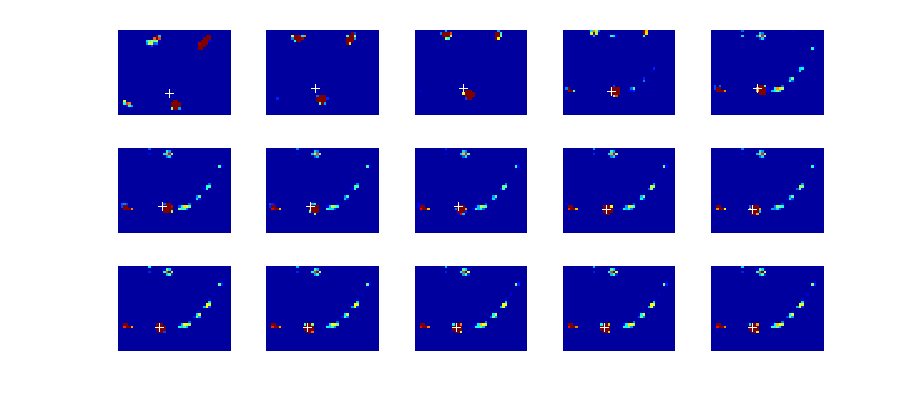
\includegraphics[width=150mm]{./eps/probing.png}}
  \caption[A series of saliency probing]{A series of saliency probing, one of those got the highest recognition score, is shown. From the left to the right, and from the top to the bottom, time goes with an interval of 100 ms (so, total length is 1500 ms). Each box represents a saliency map, the more reddish represents the higher saliency and the more bluish represents the lower saliency. The white cross represents the gaze position of the participant. As time goes, the eye gaze tracks down the highest saliency point (first row) and moves slowly in accordance with shifting of saliency map due to displacement of scene camera (second and third rows).}
  \label{fig:probing}
\end{figure*}

Interestingly, the fixation duration, which was longer than 1400 ms, negatively correlated with the score, though the standard error of that was relatively high. 

The assessment of the model is shown in Table~\ref{tab:lr-goodness}. The number of observation was 88 since each of 11 participants rates 8 long fixated movie clips, respectively. The other models, like logistic regression and non-linear regression, are also examined, but they did not explain better than the linear model.

\begin{table}[ht]
\begin{center} 
\caption{Assessment of the linear regression model.} 
\vskip 0.12in
\label{tab:lr-goodness} 
\begin{tabular}{ll} 
\hline
Attribute   & Value \\ 
\hline
\# of observations & 88 \\
Error degree of freedom & 85 \\
RMSE & 1.34 \\
$R^{2}$ & 0.106 \\
Adjusted $R^{2}$ & 0.0847 \\
F-statistics vs. constant model & 5.02 (p-value = 0.00866) \\
\hline
\end{tabular} 
\end{center} 
\end{table}

\chapter{Discussions}

The marginal distribution of the fixation duration shows the characteristics of the response toward the visual stimuli. The shape of the marginal distribution of fixation duration can be estimated as the exponential function though the marginal distribution of the reading fixation durations is illustrated as a left-skewed normal distribution, peaking at 180 ms. Then why are reading and watching so different from each other in this property? The first thing to consider is the difference of the cognitive process during the fixation. Simply put, reading involves the visual processing in addition to the lexical processing. The visual process captures the letters through the retina, Lateral Geniculate Nucleus (LGN) and the primary visual cortex. Then the information of the letters is directed to the distributed lexical processing areas. Though skipping is occasionally occurred while reading, those serial processes take a bit of latency time. Since reading is an active task, the decision for when to move and where to move to a next word, is actively and consciously made compared to watching task, those latencies tend to be preserved the normative shape. Whereas, watching the video has a different condition. The lexical processes are typically unnecessary, which are heavy tasks in time. Also the video stimuli are passive in regard to the temporal aspect. Therefore the generation of the long fixation duration is sufficiently constrained by the duration of the stimulus and the content of the stimulus at the same time. 

We recap the visual constraints which trigger the long fixation durations as three types in Table~\ref{tab:long-fixation-types}. The \textit{alerted} is an ongoing urgent situation that makes the eyes fixates an object which is thought to be a cause or a factor. This type potentially induces the emotional arousal. The second type is the \textit{successive}. It seems that the successive appearing of the objects keeps the fixation longer. However, with regard to the interpretation of that, the successive absence of the other attracting elements just lets the persistency of fixation also possible. The \textit{stationary} shows indifferent movie clips and there is no significant change. Many movie clips show calm and relaxed or depressed situation. Emotionally, the opposite of \textit{alerted}. After all, what is the meaning of the long fixation durations on the video stimuli? Despite the fact that it could be a latency time to process the cognitive information of the visual stimuli, in the other perspective, it could be waiting time to the potentially salient moment on that eye position. The waiting on the prospective location for a dramatic change or a new event is an efficient way of information processing.

Though the long fixation itself does not describe the presence of the cognitive process to memorize, in the condition of the long fixation, the arousal effect is remarkable compared to the others in the condition of the short fixation. As discussed before, the long fixation is induced by active taking or passive exposure. Since the cause of the long fixation is relatively well established by those two factors, the arousal effect on the long fixation is noticeable, but because the cause of the short fixation is complex and vague, the arousal effect on the short fixation is not observable.

The characteristics of the eye movement on the arousal effect are probed by the statistical method and the computational attention model. First of all, we hypothesize that the variation of gaze points indicates the observable response of the arousal effect in the condition of the long fixation. As we report in Section~\nameref{subsec:gaze-variations}, the gaze variation on the alerted movie clips is smaller than those on the other case, when the window size is shorter than 200 ms, to minimize the variation from the slow pursuit. Yet, the gaze variation does not have a statistical power to predict on the score, which is the measurement for the long-term memory. Though the arousal stimuli are associated with the long-term memory \cite{Cahill1996amyg,Cahill1998baso}, we conclude that the gaze variation partly explains only for the arousal effect, not for the further cognitive process, like memorization.

Second, we establish the linear model to predict the score using the computational attention model \cite{itti1998model} in addition to the fixation duration. For the short fixated movie clips, we cannot find the predicting variables, so, only the observed data of the long fixated movie clips are used. This is the backward study of Itti (2006)’s work \cite{Itti2006}, which investigates the fitness of the model to human gaze, whereas our study uses the model to evaluate the attentiveness of human. In machine learning, Zou et al. (2012) reported that stimulated fixations help to capture the useful invariant features in the image recognition task \cite{Zou2012}. This gives a hint that how it works from a computational perspective.

Although we formulate the simple method via summation of saliency scores, the method shows the significant level for the prediction. The representation of saliency map is also found in the neuronal structures \cite{Fecteau2006}, which have a peak activity in the physically salient position. And, for the fixation durations longer than 1400 ms, the longer fixated movie clips are the lesser recognized. This suggests the interpretative possibility of that the power of saliency probing tends to diminish as the fixation duration is behind time.

The value of the adjusted $R^{2}$ for the model reminds that the information of eye movement should be carefully used to estimate the cognitive process. There is the limitation of the analysis coverage, because the majority of the eye movement is the short fixated ones. 

Therefore, the investigation is not complete. We look forward to having more distinct features. A temporal modeling using the salient detectors \cite{marr1980,canny1986} and the optic flow \cite{koenderink1986} may be a promising option. Moreover, the cognitive modeling for the scene comprehension, which is related to the emotion-based reaction, guides us into the diffent level of a methodological stage. 

As discussed, the long fixations are constrained by the visual content of the video stimuli, and with regard to that, the eye movements are planned in a reciprocal manner \cite{zhang2013}. The estimation of the eye movement is viable on top of a reciprocally anticipatory model \cite{robert1985anticipatory}. The serial information of the fixation positions can be used to parsimoniously select the portion of visual features on the scene for an application using the features, and, it can be a methodological breakthrough for the cognitive modeling on the endless stream of the visual information.


\chapter{Conclusions}

We study the characteristics of the eye movements through the marginal distribution of fixation durations. We notice that the marginal distribution of fixation durations for the video stimuli has the form which is different from that of fixation durations for the reading materials. The behavioral basis for the difference may attribute to the lighter load for the cognitive process and the temporal and spatial constraints which are given by the video stimuli. Those constraints are summed up as three distinctive types: alerted, successive and stationary. We find the arousal effect only for the long fixated movie clips. The small gaze variation for the long fixation indicates an active response to the arousal stimuli. However, the gaze variation does not help to estimate for the score, and, among the long fixations, just the fixation duration and the saliency-probing activity are significant to model. We can appreciate this computational model within the embodied cognitive framework with the perception-action cycling.



\bibliographystyle{IEEEtran}
\bibliography{kim2014msthesis}

\keywordalt{안구 운동, 응시, 시공간, 장기 기억, 계산학적 모델링}
\begin{abstractalt}
안구 운동은 뇌 활동을 관찰할 수 있는 비침습적이면서 활용도가 높은 지표이다. 이러한 배경으로 최근 안경류 웨어러블 장비가 연구 기관을 중심으로 빠르게 보급되고 있으며 안구 운동에 대한 연구 활동과 관련 산업의 성장을 고도화 하고 있다. 우리는 아동용 비디오 시청 환경에서 안구 운동을 장기 응시와 단기 응시를 분류하여 연구해 보았다. 응시 기간에 따른 장기 기억 상관 여부를 확인해 보았지만 유의성을 발견할 수 없었다. 하지만 시청 자극을 주의 상황과 중립 상황으로 나눈 후 응시 기간에 따른 차이를 확인 하였을 때 긴 응시에서는 장기 기억 인출에서 통계적으로 유의미한 차이를 발견할 수 있었지만 짧은 응시에서는 그렇지 못하였다. 이를 바탕으로 관측된 안구 운동에 대한 계산학적인 방법인 현저점 탐색과 응시 길이를 이용한 선형 회귀 모델을 제안하고 평가하였다. 이러한 안구 운동의 특징에서 발견되는 장기 기억과 관련된 인지 처리 과정은 평생 학습 기제에서 선택적 주의를 통한 효율성 추구가 제한된 인지 처리 능력 안에서 중요한 요소로 기여함을 시사한다.
\end{abstractalt}

\acknowledgement
Thanks to Prof. Sungryong Koh and our colleagues, Eun-Sol Kim, Kyoung-Woon On and Kyung-Jae Lee for helpful comments to improve experimental analyses.

This work was supported by the National Research Foundation of Korea (NRF) grant funded by the Korea government (MSIP) (NRF-2010-0017734-Videome),
supported in part by ICT R\&D program funded by the Korea government (MSIP/IITP) (10035348-mLife, 14-824-09-014, 10044009-HRI.MESSI).

\end{document}

